\documentclass[1p]{elsarticle_modified}
%\bibliographystyle{elsarticle-num}

%\usepackage[colorlinks]{hyperref}
%\usepackage{abbrmath_seonhwa} %\Abb, \Ascr, \Acal ,\Abf, \Afrak
\usepackage{amsfonts}
\usepackage{amssymb}
\usepackage{amsmath}
\usepackage{amsthm}
\usepackage{scalefnt}
\usepackage{amsbsy}
\usepackage{kotex}
\usepackage{caption}
\usepackage{subfig}
\usepackage{color}
\usepackage{graphicx}
\usepackage{xcolor} %% white, black, red, green, blue, cyan, magenta, yellow
\usepackage{float}
\usepackage{setspace}
\usepackage{hyperref}

\usepackage{tikz}
\usetikzlibrary{arrows}

\usepackage{multirow}
\usepackage{array} % fixed length table
\usepackage{hhline}

%%%%%%%%%%%%%%%%%%%%%
\makeatletter
\renewcommand*\env@matrix[1][\arraystretch]{%
	\edef\arraystretch{#1}%
	\hskip -\arraycolsep
	\let\@ifnextchar\new@ifnextchar
	\array{*\c@MaxMatrixCols c}}
\makeatother %https://tex.stackexchange.com/questions/14071/how-can-i-increase-the-line-spacing-in-a-matrix
%%%%%%%%%%%%%%%

\usepackage[normalem]{ulem}

\newcommand{\msout}[1]{\ifmmode\text{\sout{\ensuremath{#1}}}\else\sout{#1}\fi}
%SOURCE: \msout is \stkout macro in https://tex.stackexchange.com/questions/20609/strikeout-in-math-mode

\newcommand{\cancel}[1]{
	\ifmmode
	{\color{red}\msout{#1}}
	\else
	{\color{red}\sout{#1}}
	\fi
}

\newcommand{\add}[1]{
	{\color{blue}\uwave{#1}}
}

\newcommand{\replace}[2]{
	\ifmmode
	{\color{red}\msout{#1}}{\color{blue}\uwave{#2}}
	\else
	{\color{red}\sout{#1}}{\color{blue}\uwave{#2}}
	\fi
}

\newcommand{\Sol}{\mathcal{S}} %segment
\newcommand{\D}{D} %diagram
\newcommand{\A}{\mathcal{A}} %arc


%%%%%%%%%%%%%%%%%%%%%%%%%%%%%5 test

\def\sl{\operatorname{\textup{SL}}(2,\Cbb)}
\def\psl{\operatorname{\textup{PSL}}(2,\Cbb)}
\def\quan{\mkern 1mu \triangleright \mkern 1mu}

\theoremstyle{definition}
\newtheorem{thm}{Theorem}[section]
\newtheorem{prop}[thm]{Proposition}
\newtheorem{lem}[thm]{Lemma}
\newtheorem{ques}[thm]{Question}
\newtheorem{cor}[thm]{Corollary}
\newtheorem{defn}[thm]{Definition}
\newtheorem{exam}[thm]{Example}
\newtheorem{rmk}[thm]{Remark}
\newtheorem{alg}[thm]{Algorithm}

\newcommand{\I}{\sqrt{-1}}
\begin{document}

%\begin{frontmatter}
%
%\title{Boundary parabolic representations of knots up to 8 crossings}
%
%%% Group authors per affiliation:
%\author{Yunhi Cho} 
%\address{Department of Mathematics, University of Seoul, Seoul, Korea}
%\ead{yhcho@uos.ac.kr}
%
%
%\author{Seonhwa Kim} %\fnref{s_kim}}
%\address{Center for Geometry and Physics, Institute for Basic Science, Pohang, 37673, Korea}
%\ead{ryeona17@ibs.re.kr}
%
%\author{Hyuk Kim}
%\address{Department of Mathematical Sciences, Seoul National University, Seoul 08826, Korea}
%\ead{hyukkim@snu.ac.kr}
%
%\author{Seokbeom Yoon}
%\address{Department of Mathematical Sciences, Seoul National University, Seoul, 08826,  Korea}
%\ead{sbyoon15@snu.ac.kr}
%
%\begin{abstract}
%We find all boundary parabolic representation of knots up to 8 crossings.
%
%\end{abstract}
%\begin{keyword}
%    \MSC[2010] 57M25 
%\end{keyword}
%
%\end{frontmatter}

%\linenumbers
%\tableofcontents
%
\newcommand\colored[1]{\textcolor{white}{\rule[-0.35ex]{0.8em}{1.4ex}}\kern-0.8em\color{red} #1}%
%\newcommand\colored[1]{\textcolor{white}{ #1}\kern-2.17ex	\textcolor{white}{ #1}\kern-1.81ex	\textcolor{white}{ #1}\kern-2.15ex\color{red}#1	}

{\Large $\underline{11n_{153}~(K11n_{153})}$}

\setlength{\tabcolsep}{10pt}
\renewcommand{\arraystretch}{1.6}
\vspace{1cm}\begin{tabular}{m{100pt}>{\centering\arraybackslash}m{274pt}}
\multirow{5}{120pt}{
	\centering
	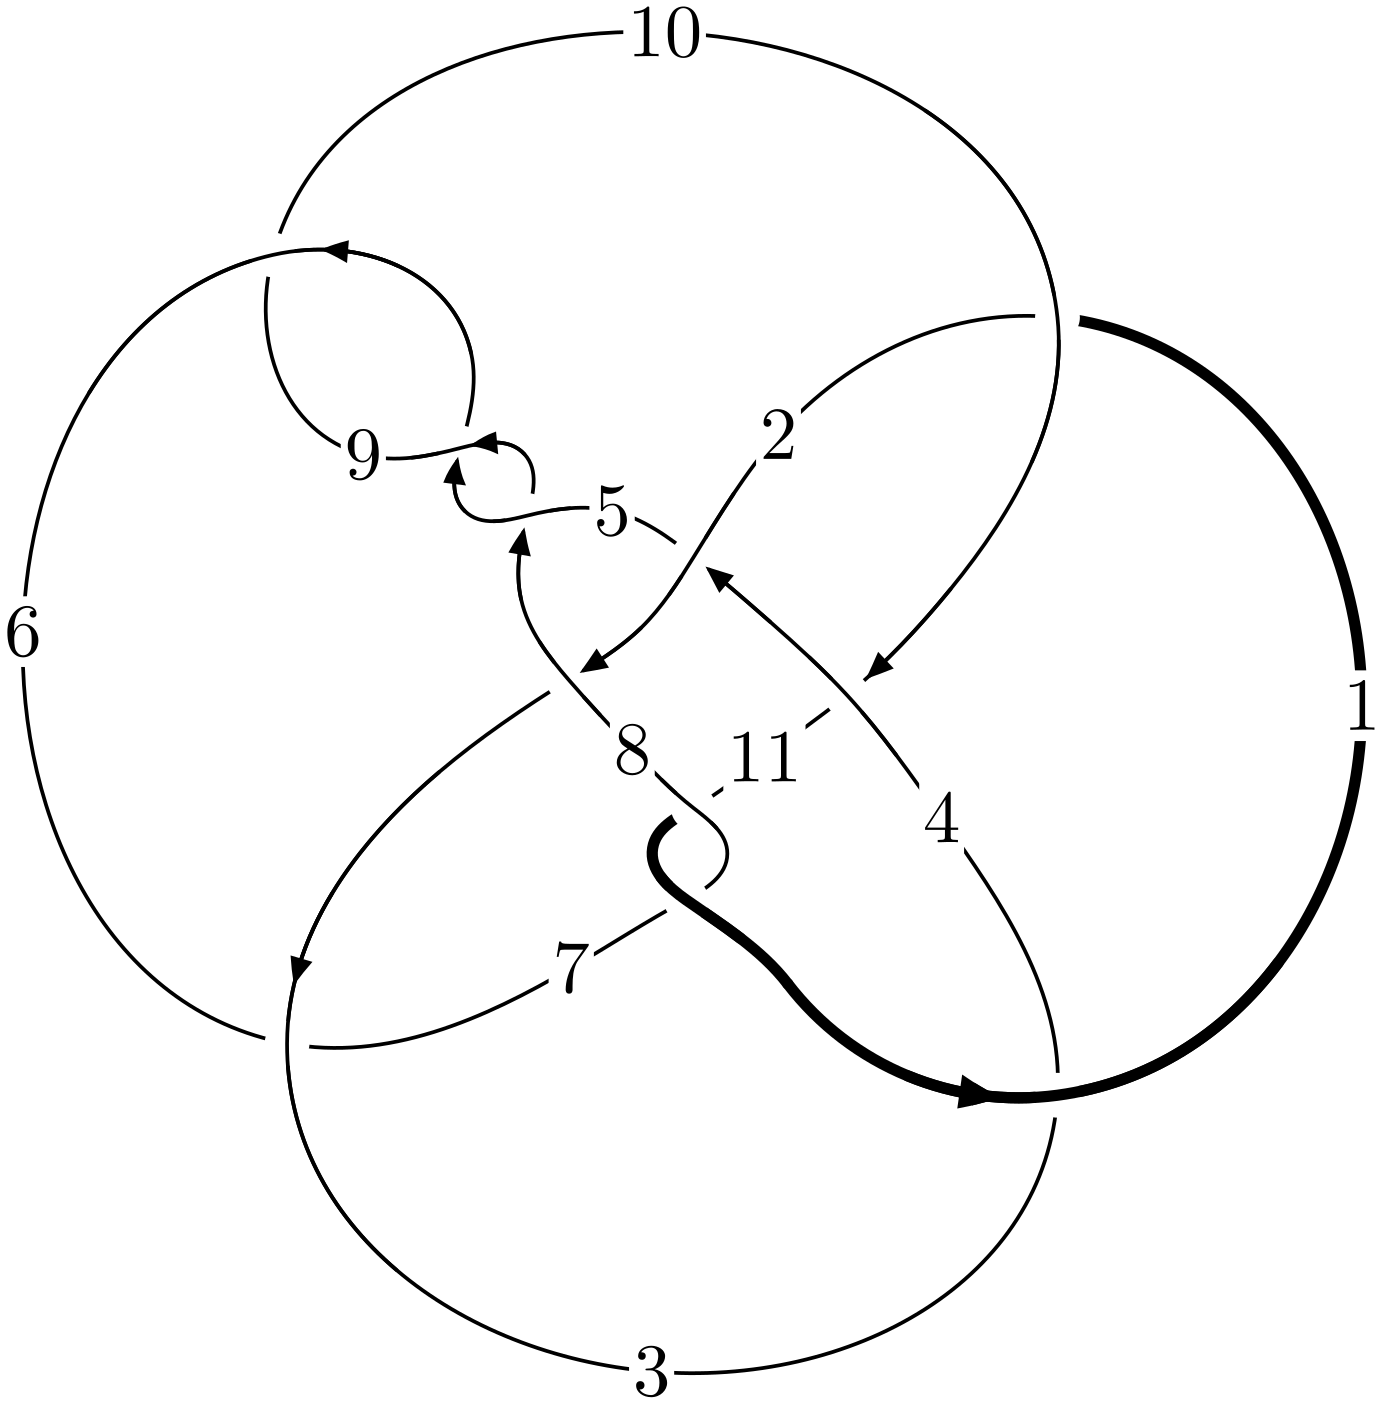
\includegraphics[width=112pt]{../../../GIT/diagram.site/Diagrams/png/769_11n_153.png}\\
\ \ \ A knot diagram\footnotemark}&
\allowdisplaybreaks
\textbf{Linearized knot diagam} \\
\cline{2-2}
 &
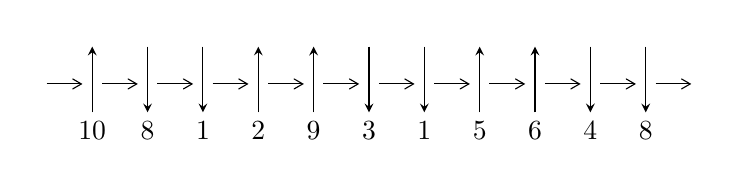
\begin{tikzpicture}[x=20pt, y=17pt]
	% nodes
	\node (C0) at (0, 0) {};
	\node (C1) at (1, 0) {};
	\node (C1U) at (1, +1) {};
	\node (C1D) at (1, -1) {10};

	\node (C2) at (2, 0) {};
	\node (C2U) at (2, +1) {};
	\node (C2D) at (2, -1) {8};

	\node (C3) at (3, 0) {};
	\node (C3U) at (3, +1) {};
	\node (C3D) at (3, -1) {1};

	\node (C4) at (4, 0) {};
	\node (C4U) at (4, +1) {};
	\node (C4D) at (4, -1) {2};

	\node (C5) at (5, 0) {};
	\node (C5U) at (5, +1) {};
	\node (C5D) at (5, -1) {9};

	\node (C6) at (6, 0) {};
	\node (C6U) at (6, +1) {};
	\node (C6D) at (6, -1) {3};

	\node (C7) at (7, 0) {};
	\node (C7U) at (7, +1) {};
	\node (C7D) at (7, -1) {1};

	\node (C8) at (8, 0) {};
	\node (C8U) at (8, +1) {};
	\node (C8D) at (8, -1) {5};

	\node (C9) at (9, 0) {};
	\node (C9U) at (9, +1) {};
	\node (C9D) at (9, -1) {6};

	\node (C10) at (10, 0) {};
	\node (C10U) at (10, +1) {};
	\node (C10D) at (10, -1) {4};

	\node (C11) at (11, 0) {};
	\node (C11U) at (11, +1) {};
	\node (C11D) at (11, -1) {8};
	\node (C12) at (12, 0) {};

	% arrows
	\draw[->,>={angle 60}]
	(C0) edge (C1) (C1) edge (C2) (C2) edge (C3) (C3) edge (C4) (C4) edge (C5) (C5) edge (C6) (C6) edge (C7) (C7) edge (C8) (C8) edge (C9) (C9) edge (C10) (C10) edge (C11) (C11) edge (C12) ;	\draw[->,>=stealth]
	(C1D) edge (C1U) (C2U) edge (C2D) (C3U) edge (C3D) (C4D) edge (C4U) (C5D) edge (C5U) (C6U) edge (C6D) (C7U) edge (C7D) (C8D) edge (C8U) (C9D) edge (C9U) (C10U) edge (C10D) (C11U) edge (C11D) ;
	\end{tikzpicture} \\
\hhline{~~} \\& 
\textbf{Solving Sequence} \\ \cline{2-2} 
 &
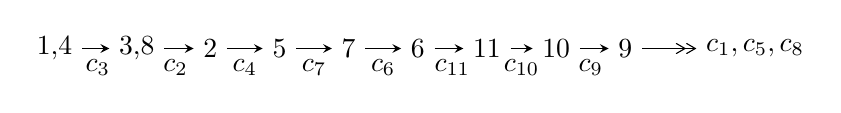
\begin{tikzpicture}[x=25pt, y=7pt]
	% node
	\node (A0) at (-1/8, 0) {1,4};
	\node (A1) at (17/16, 0) {3,8};
	\node (A2) at (17/8, 0) {2};
	\node (A3) at (25/8, 0) {5};
	\node (A4) at (33/8, 0) {7};
	\node (A5) at (41/8, 0) {6};
	\node (A6) at (49/8, 0) {11};
	\node (A7) at (57/8, 0) {10};
	\node (A8) at (65/8, 0) {9};
	\node (C1) at (1/2, -1) {$c_{3}$};
	\node (C2) at (13/8, -1) {$c_{2}$};
	\node (C3) at (21/8, -1) {$c_{4}$};
	\node (C4) at (29/8, -1) {$c_{7}$};
	\node (C5) at (37/8, -1) {$c_{6}$};
	\node (C6) at (45/8, -1) {$c_{11}$};
	\node (C7) at (53/8, -1) {$c_{10}$};
	\node (C8) at (61/8, -1) {$c_{9}$};
	\node (A9) at (10, 0) {$c_{1},c_{5},c_{8}$};

	% edge
	\draw[->,>=stealth]	
	(A0) edge (A1) (A1) edge (A2) (A2) edge (A3) (A3) edge (A4) (A4) edge (A5) (A5) edge (A6) (A6) edge (A7) (A7) edge (A8) ;
	\draw[->>,>={angle 60}]	
	(A8) edge (A9);
\end{tikzpicture} \\ 

\end{tabular} \\

\footnotetext{
The image of knot diagram is generated by the software ``\textbf{Draw programme}" developed by Andrew Bartholomew(\url{http://www.layer8.co.uk/maths/draw/index.htm\#Running-draw}), where we modified some parts for our purpose(\url{https://github.com/CATsTAILs/LinksPainter}).
}\phantom \\ \newline 
\centering \textbf{Ideals for irreducible components\footnotemark of $X_{\text{par}}$} 
 
\begin{align*}
I^u_{1}&=\langle 
-969784110565 u^{17}+7522067922888 u^{16}+\cdots+3213286025447 b-9008416143977,\\
\phantom{I^u_{1}}&\phantom{= \langle  }9008416143977 u^{17}-73317472411273 u^{16}+\cdots+25706288203576 a-26276930799793,\\
\phantom{I^u_{1}}&\phantom{= \langle  }u^{18}-9 u^{17}+\cdots-33 u-8\rangle \\
I^u_{2}&=\langle 
- u^2+b- u,\;a- u-1,\;u^5+3 u^4+3 u^3+2 u^2+u+1\rangle \\
I^u_{3}&=\langle 
- u^8-7 u^7-17 u^6-12 u^5+13 u^4+16 u^3- a u-10 u^2+b-10 u+5,\;15 u^8 a+8 u^8+\cdots-75 a-70,\\
\phantom{I^u_{3}}&\phantom{= \langle  }u^9+7 u^8+16 u^7+7 u^6-19 u^5-11 u^4+20 u^3+6 u^2-11 u+3\rangle \\
I^u_{4}&=\langle 
u^2+b+2 u+1,\;- u^2+a-2 u,\;u^3+3 u^2+2 u+1\rangle \\
\\
\end{align*}
\raggedright * 4 irreducible components of $\dim_{\mathbb{C}}=0$, with total 44 representations.\\
\footnotetext{All coefficients of polynomials are rational numbers. But the coefficients are sometimes approximated in decimal forms when there is not enough margin.}
\newpage
\renewcommand{\arraystretch}{1}
\centering \section*{I. $I^u_{1}= \langle -9.70\times10^{11} u^{17}+7.52\times10^{12} u^{16}+\cdots+3.21\times10^{12} b-9.01\times10^{12},\;9.01\times10^{12} u^{17}-7.33\times10^{13} u^{16}+\cdots+2.57\times10^{13} a-2.63\times10^{13},\;u^{18}-9 u^{17}+\cdots-33 u-8 \rangle$}
\flushleft \textbf{(i) Arc colorings}\\
\begin{tabular}{m{7pt} m{180pt} m{7pt} m{180pt} }
\flushright $a_{1}=$&$\begin{pmatrix}0\\u\end{pmatrix}$ \\
\flushright $a_{4}=$&$\begin{pmatrix}1\\0\end{pmatrix}$ \\
\flushright $a_{3}=$&$\begin{pmatrix}1\\- u^2\end{pmatrix}$ \\
\flushright $a_{8}=$&$\begin{pmatrix}-0.350436 u^{17}+2.85212 u^{16}+\cdots-14.9807 u+1.02220\\0.301804 u^{17}-2.34093 u^{16}+\cdots+10.5422 u+2.80349\end{pmatrix}$ \\
\flushright $a_{2}=$&$\begin{pmatrix}0.0586285 u^{17}-0.559036 u^{16}+\cdots+4.76685 u-1.68018\\0.0313795 u^{17}-0.210283 u^{16}+\cdots+0.745441 u-0.469028\end{pmatrix}$ \\
\flushright $a_{5}=$&$\begin{pmatrix}0.0993811 u^{17}-0.841718 u^{16}+\cdots+4.58790 u+0.0398829\\0.0313795 u^{17}-0.210283 u^{16}+\cdots-0.254559 u-0.469028\end{pmatrix}$ \\
\flushright $a_{7}=$&$\begin{pmatrix}-0.350436 u^{17}+2.85212 u^{16}+\cdots-14.9807 u+1.02220\\0.677118 u^{17}-5.29868 u^{16}+\cdots+23.3052 u+5.21793\end{pmatrix}$ \\
\flushright $a_{6}=$&$\begin{pmatrix}-0.0486318 u^{17}+0.511195 u^{16}+\cdots-4.43851 u+3.82569\\0.257046 u^{17}-1.94618 u^{16}+\cdots+8.50546 u+2.21542\end{pmatrix}$ \\
\flushright $a_{11}=$&$\begin{pmatrix}0.291572 u^{17}-2.39120 u^{16}+\cdots+14.0411 u-0.347607\\-0.232943 u^{17}+1.83217 u^{16}+\cdots-8.27426 u-2.33257\end{pmatrix}$ \\
\flushright $a_{10}=$&$\begin{pmatrix}0.0586285 u^{17}-0.559036 u^{16}+\cdots+5.76685 u-2.68018\\-0.232943 u^{17}+1.83217 u^{16}+\cdots-8.27426 u-2.33257\end{pmatrix}$ \\
\flushright $a_{9}=$&$\begin{pmatrix}-0.00591672 u^{17}+0.133324 u^{16}+\cdots-1.44739 u+2.47523\\-0.0460630 u^{17}+0.308887 u^{16}+\cdots+0.724360 u+0.154459\end{pmatrix}$\\ \flushright $a_{9}=$&$\begin{pmatrix}-0.00591672 u^{17}+0.133324 u^{16}+\cdots-1.44739 u+2.47523\\-0.0460630 u^{17}+0.308887 u^{16}+\cdots+0.724360 u+0.154459\end{pmatrix}$\\&\end{tabular}
\flushleft \textbf{(ii) Obstruction class $= -1$}\\~\\
\flushleft \textbf{(iii) Cusp Shapes $= \frac{3008625095462}{3213286025447} u^{17}-\frac{22676683370184}{3213286025447} u^{16}+\cdots+\frac{74739485745112}{3213286025447} u+\frac{16280782342958}{3213286025447}$}\\~\\
\newpage\renewcommand{\arraystretch}{1}
\flushleft \textbf{(iv) u-Polynomials at the component}\newline \\
\begin{tabular}{m{50pt}|m{274pt}}
Crossings & \hspace{64pt}u-Polynomials at each crossing \\
\hline $$\begin{aligned}c_{1},c_{4}\end{aligned}$$&$\begin{aligned}
&u^{18}+2 u^{17}+\cdots-2 u+1
\end{aligned}$\\
\hline $$\begin{aligned}c_{2}\end{aligned}$$&$\begin{aligned}
&u^{18}-2 u^{16}+\cdots-5 u-1
\end{aligned}$\\
\hline $$\begin{aligned}c_{3}\end{aligned}$$&$\begin{aligned}
&u^{18}-9 u^{17}+\cdots-33 u-8
\end{aligned}$\\
\hline $$\begin{aligned}c_{5},c_{8},c_{9}\end{aligned}$$&$\begin{aligned}
&u^{18}-6 u^{17}+\cdots+3 u+2
\end{aligned}$\\
\hline $$\begin{aligned}c_{6},c_{7},c_{11}\end{aligned}$$&$\begin{aligned}
&u^{18}-13 u^{16}+\cdots- u+1
\end{aligned}$\\
\hline $$\begin{aligned}c_{10}\end{aligned}$$&$\begin{aligned}
&u^{18}+17 u^{17}+\cdots+4352 u+512
\end{aligned}$\\
\hline
\end{tabular}\\~\\
\newpage\renewcommand{\arraystretch}{1}
\flushleft \textbf{(v) Riley Polynomials at the component}\newline \\
\begin{tabular}{m{50pt}|m{274pt}}
Crossings & \hspace{64pt}Riley Polynomials at each crossing \\
\hline $$\begin{aligned}c_{1},c_{4}\end{aligned}$$&$\begin{aligned}
&y^{18}+2 y^{17}+\cdots-2 y+1
\end{aligned}$\\
\hline $$\begin{aligned}c_{2}\end{aligned}$$&$\begin{aligned}
&y^{18}-4 y^{17}+\cdots-35 y+1
\end{aligned}$\\
\hline $$\begin{aligned}c_{3}\end{aligned}$$&$\begin{aligned}
&y^{18}-13 y^{17}+\cdots-2017 y+64
\end{aligned}$\\
\hline $$\begin{aligned}c_{5},c_{8},c_{9}\end{aligned}$$&$\begin{aligned}
&y^{18}-18 y^{17}+\cdots+35 y+4
\end{aligned}$\\
\hline $$\begin{aligned}c_{6},c_{7},c_{11}\end{aligned}$$&$\begin{aligned}
&y^{18}-26 y^{17}+\cdots-7 y+1
\end{aligned}$\\
\hline $$\begin{aligned}c_{10}\end{aligned}$$&$\begin{aligned}
&y^{18}- y^{17}+\cdots+458752 y+262144
\end{aligned}$\\
\hline
\end{tabular}\\~\\
\newpage\flushleft \textbf{(vi) Complex Volumes and Cusp Shapes}
$$\begin{array}{c|c|c}  
\text{Solutions to }I^u_{1}& \I (\text{vol} + \sqrt{-1}CS) & \text{Cusp shape}\\
 \hline 
\begin{aligned}
u &= \phantom{-}0.843032 + 0.524058 I \\
a &= -0.586941 + 1.246720 I \\
b &= \phantom{-}1.148160 - 0.743433 I\end{aligned}
 & \phantom{-}2.18663 - 2.73072 I & \phantom{-}12.5447 + 6.6202 I \\ \hline\begin{aligned}
u &= \phantom{-}0.843032 - 0.524058 I \\
a &= -0.586941 - 1.246720 I \\
b &= \phantom{-}1.148160 + 0.743433 I\end{aligned}
 & \phantom{-}2.18663 + 2.73072 I & \phantom{-}12.5447 - 6.6202 I \\ \hline\begin{aligned}
u &= \phantom{-}1.09266\phantom{ +0.000000I} \\
a &= -1.66916\phantom{ +0.000000I} \\
b &= \phantom{-}1.82383\phantom{ +0.000000I}\end{aligned}
 & \phantom{-}2.25932\phantom{ +0.000000I} & \phantom{-}7.45690\phantom{ +0.000000I} \\ \hline\begin{aligned}
u &= -0.926749 + 0.681554 I \\
a &= \phantom{-}0.358863 - 0.335448 I \\
b &= \phantom{-}0.103949 - 0.555460 I\end{aligned}
 & \phantom{-}3.08255 + 2.45502 I & \phantom{-}4.56614 - 2.39715 I \\ \hline\begin{aligned}
u &= -0.926749 - 0.681554 I \\
a &= \phantom{-}0.358863 + 0.335448 I \\
b &= \phantom{-}0.103949 + 0.555460 I\end{aligned}
 & \phantom{-}3.08255 - 2.45502 I & \phantom{-}4.56614 + 2.39715 I \\ \hline\begin{aligned}
u &= -0.439225 + 1.123520 I \\
a &= -0.064923 + 0.354238 I \\
b &= \phantom{-}0.369476 + 0.228533 I\end{aligned}
 & \phantom{-}0.29930 + 2.83434 I & -6.26246 - 4.02020 I \\ \hline\begin{aligned}
u &= -0.439225 - 1.123520 I \\
a &= -0.064923 - 0.354238 I \\
b &= \phantom{-}0.369476 - 0.228533 I\end{aligned}
 & \phantom{-}0.29930 - 2.83434 I & -6.26246 + 4.02020 I \\ \hline\begin{aligned}
u &= -0.305459 + 0.432561 I \\
a &= -0.854284 - 0.273373 I \\
b &= -0.379199 + 0.286025 I\end{aligned}
 & -0.589102 + 1.103260 I & -3.61302 - 5.14507 I \\ \hline\begin{aligned}
u &= -0.305459 - 0.432561 I \\
a &= -0.854284 + 0.273373 I \\
b &= -0.379199 - 0.286025 I\end{aligned}
 & -0.589102 - 1.103260 I & -3.61302 + 5.14507 I \\ \hline\begin{aligned}
u &= \phantom{-}1.56461 + 0.17007 I \\
a &= \phantom{-}1.212670 + 0.097343 I \\
b &= -1.88079 - 0.35855 I\end{aligned}
 & -6.68818 - 3.40005 I & -2.59654 + 3.50270 I\\
 \hline 
 \end{array}$$\newpage$$\begin{array}{c|c|c}  
\text{Solutions to }I^u_{1}& \I (\text{vol} + \sqrt{-1}CS) & \text{Cusp shape}\\
 \hline 
\begin{aligned}
u &= \phantom{-}1.56461 - 0.17007 I \\
a &= \phantom{-}1.212670 - 0.097343 I \\
b &= -1.88079 + 0.35855 I\end{aligned}
 & -6.68818 + 3.40005 I & -2.59654 - 3.50270 I \\ \hline\begin{aligned}
u &= -0.32355 + 1.54849 I \\
a &= \phantom{-}0.154189 - 0.448176 I \\
b &= -0.644108 - 0.383768 I\end{aligned}
 & \phantom{-}5.90785 + 4.79162 I & \phantom{-}2.11811 - 3.69242 I \\ \hline\begin{aligned}
u &= -0.32355 - 1.54849 I \\
a &= \phantom{-}0.154189 + 0.448176 I \\
b &= -0.644108 + 0.383768 I\end{aligned}
 & \phantom{-}5.90785 - 4.79162 I & \phantom{-}2.11811 + 3.69242 I \\ \hline\begin{aligned}
u &= \phantom{-}1.77246 + 0.37808 I \\
a &= -1.060540 + 0.004179 I \\
b &= \phantom{-}1.88134 + 0.39356 I\end{aligned}
 & -7.47923 - 8.86125 I & -3.00235 + 6.30100 I \\ \hline\begin{aligned}
u &= \phantom{-}1.77246 - 0.37808 I \\
a &= -1.060540 - 0.004179 I \\
b &= \phantom{-}1.88134 - 0.39356 I\end{aligned}
 & -7.47923 + 8.86125 I & -3.00235 - 6.30100 I \\ \hline\begin{aligned}
u &= -0.177652\phantom{ +0.000000I} \\
a &= \phantom{-}4.24705\phantom{ +0.000000I} \\
b &= \phantom{-}0.754498\phantom{ +0.000000I}\end{aligned}
 & \phantom{-}3.37072\phantom{ +0.000000I} & \phantom{-}0.911940\phantom{ +0.000000I} \\ \hline\begin{aligned}
u &= \phantom{-}1.85738 + 0.59535 I \\
a &= \phantom{-}0.989524 - 0.084101 I \\
b &= -1.88799 - 0.43291 I\end{aligned}
 & -1.17978 - 13.07450 I & \phantom{-}0.56098 + 6.39967 I \\ \hline\begin{aligned}
u &= \phantom{-}1.85738 - 0.59535 I \\
a &= \phantom{-}0.989524 + 0.084101 I \\
b &= -1.88799 + 0.43291 I\end{aligned}
 & -1.17978 + 13.07450 I & \phantom{-}0.56098 - 6.39967 I\\
 \hline 
 \end{array}$$\newpage\newpage\renewcommand{\arraystretch}{1}
\centering \section*{II. $I^u_{2}= \langle - u^2+b- u,\;a- u-1,\;u^5+3 u^4+3 u^3+2 u^2+u+1 \rangle$}
\flushleft \textbf{(i) Arc colorings}\\
\begin{tabular}{m{7pt} m{180pt} m{7pt} m{180pt} }
\flushright $a_{1}=$&$\begin{pmatrix}0\\u\end{pmatrix}$ \\
\flushright $a_{4}=$&$\begin{pmatrix}1\\0\end{pmatrix}$ \\
\flushright $a_{3}=$&$\begin{pmatrix}1\\- u^2\end{pmatrix}$ \\
\flushright $a_{8}=$&$\begin{pmatrix}u+1\\u^2+u\end{pmatrix}$ \\
\flushright $a_{2}=$&$\begin{pmatrix}- u^4-3 u^3-3 u^2- u+1\\u+1\end{pmatrix}$ \\
\flushright $a_{5}=$&$\begin{pmatrix}u^4+3 u^3+2 u^2- u-1\\- u^2-2 u-1\end{pmatrix}$ \\
\flushright $a_{7}=$&$\begin{pmatrix}u+1\\- u^3+u\end{pmatrix}$ \\
\flushright $a_{6}=$&$\begin{pmatrix}u^2+2 u+1\\- u^4-2 u^3+u\end{pmatrix}$ \\
\flushright $a_{11}=$&$\begin{pmatrix}u^3+2 u^2+u\\u^4+2 u^3+u^2+u\end{pmatrix}$ \\
\flushright $a_{10}=$&$\begin{pmatrix}u^4+3 u^3+3 u^2+2 u\\u^4+2 u^3+u^2+u\end{pmatrix}$ \\
\flushright $a_{9}=$&$\begin{pmatrix}u^4+2 u^3- u-2\\- u^3-2 u^2-2 u-2\end{pmatrix}$\\ \flushright $a_{9}=$&$\begin{pmatrix}u^4+2 u^3- u-2\\- u^3-2 u^2-2 u-2\end{pmatrix}$\\&\end{tabular}
\flushleft \textbf{(ii) Obstruction class $= 1$}\\~\\
\flushleft \textbf{(iii) Cusp Shapes $= -7 u^4-19 u^3-16 u^2-8 u-2$}\\~\\
\newpage\renewcommand{\arraystretch}{1}
\flushleft \textbf{(iv) u-Polynomials at the component}\newline \\
\begin{tabular}{m{50pt}|m{274pt}}
Crossings & \hspace{64pt}u-Polynomials at each crossing \\
\hline $$\begin{aligned}c_{1},c_{4}\end{aligned}$$&$\begin{aligned}
&u^5-2 u^4+u^3+u^2- u+1
\end{aligned}$\\
\hline $$\begin{aligned}c_{2}\end{aligned}$$&$\begin{aligned}
&u^5+3 u^4+4 u^3+3 u^2+u+1
\end{aligned}$\\
\hline $$\begin{aligned}c_{3}\end{aligned}$$&$\begin{aligned}
&u^5+3 u^4+3 u^3+2 u^2+u+1
\end{aligned}$\\
\hline $$\begin{aligned}c_{5}\end{aligned}$$&$\begin{aligned}
&u^5- u^4-3 u^3+2 u^2+3 u-1
\end{aligned}$\\
\hline $$\begin{aligned}c_{6},c_{11}\end{aligned}$$&$\begin{aligned}
&u^5- u^3+2 u^2-2 u+1
\end{aligned}$\\
\hline $$\begin{aligned}c_{7}\end{aligned}$$&$\begin{aligned}
&u^5- u^3-2 u^2-2 u-1
\end{aligned}$\\
\hline $$\begin{aligned}c_{8},c_{9}\end{aligned}$$&$\begin{aligned}
&u^5+u^4-3 u^3-2 u^2+3 u+1
\end{aligned}$\\
\hline $$\begin{aligned}c_{10}\end{aligned}$$&$\begin{aligned}
&u^5- u^4+u^3+u^2-2 u+1
\end{aligned}$\\
\hline
\end{tabular}\\~\\
\newpage\renewcommand{\arraystretch}{1}
\flushleft \textbf{(v) Riley Polynomials at the component}\newline \\
\begin{tabular}{m{50pt}|m{274pt}}
Crossings & \hspace{64pt}Riley Polynomials at each crossing \\
\hline $$\begin{aligned}c_{1},c_{4}\end{aligned}$$&$\begin{aligned}
&y^5-2 y^4+3 y^3+y^2- y-1
\end{aligned}$\\
\hline $$\begin{aligned}c_{2}\end{aligned}$$&$\begin{aligned}
&y^5- y^4-7 y^2-5 y-1
\end{aligned}$\\
\hline $$\begin{aligned}c_{3}\end{aligned}$$&$\begin{aligned}
&y^5-3 y^4- y^3-4 y^2-3 y-1
\end{aligned}$\\
\hline $$\begin{aligned}c_{5},c_{8},c_{9}\end{aligned}$$&$\begin{aligned}
&y^5-7 y^4+19 y^3-24 y^2+13 y-1
\end{aligned}$\\
\hline $$\begin{aligned}c_{6},c_{7},c_{11}\end{aligned}$$&$\begin{aligned}
&y^5-2 y^4-3 y^3-1
\end{aligned}$\\
\hline $$\begin{aligned}c_{10}\end{aligned}$$&$\begin{aligned}
&y^5+y^4- y^3-3 y^2+2 y-1
\end{aligned}$\\
\hline
\end{tabular}\\~\\
\newpage\flushleft \textbf{(vi) Complex Volumes and Cusp Shapes}
$$\begin{array}{c|c|c}  
\text{Solutions to }I^u_{2}& \I (\text{vol} + \sqrt{-1}CS) & \text{Cusp shape}\\
 \hline 
\begin{aligned}
u &= -0.761946 + 0.720973 I \\
a &= \phantom{-}0.238054 + 0.720973 I \\
b &= -0.701186 - 0.377712 I\end{aligned}
 & \phantom{-}1.60363 + 2.70217 I & -2.62337 - 3.99219 I \\ \hline\begin{aligned}
u &= -0.761946 - 0.720973 I \\
a &= \phantom{-}0.238054 - 0.720973 I \\
b &= -0.701186 + 0.377712 I\end{aligned}
 & \phantom{-}1.60363 - 2.70217 I & -2.62337 + 3.99219 I \\ \hline\begin{aligned}
u &= \phantom{-}0.216341 + 0.655213 I \\
a &= \phantom{-}1.216340 + 0.655213 I \\
b &= -0.166160 + 0.938713 I\end{aligned}
 & \phantom{-}8.18698 + 5.82350 I & \phantom{-}7.02930 - 4.66310 I \\ \hline\begin{aligned}
u &= \phantom{-}0.216341 - 0.655213 I \\
a &= \phantom{-}1.216340 - 0.655213 I \\
b &= -0.166160 - 0.938713 I\end{aligned}
 & \phantom{-}8.18698 - 5.82350 I & \phantom{-}7.02930 + 4.66310 I \\ \hline\begin{aligned}
u &= -1.90879\phantom{ +0.000000I} \\
a &= -0.908791\phantom{ +0.000000I} \\
b &= \phantom{-}1.73469\phantom{ +0.000000I}\end{aligned}
 & -6.42175\phantom{ +0.000000I} & -5.81190\phantom{ +0.000000I}\\
 \hline 
 \end{array}$$\newpage\newpage\renewcommand{\arraystretch}{1}
\centering \section*{III. $I^u_{3}= \langle - u^8-7 u^7+\cdots+b+5,\;15 u^8 a+8 u^8+\cdots-75 a-70,\;u^9+7 u^8+\cdots-11 u+3 \rangle$}
\flushleft \textbf{(i) Arc colorings}\\
\begin{tabular}{m{7pt} m{180pt} m{7pt} m{180pt} }
\flushright $a_{1}=$&$\begin{pmatrix}0\\u\end{pmatrix}$ \\
\flushright $a_{4}=$&$\begin{pmatrix}1\\0\end{pmatrix}$ \\
\flushright $a_{3}=$&$\begin{pmatrix}1\\- u^2\end{pmatrix}$ \\
\flushright $a_{8}=$&$\begin{pmatrix}a\\u^8+7 u^7+17 u^6+12 u^5-13 u^4-16 u^3+a u+10 u^2+10 u-5\end{pmatrix}$ \\
\flushright $a_{2}=$&$\begin{pmatrix}u^7 a+\frac{1}{3} u^8+\cdots-3 a-\frac{8}{3}\\- u^7 a-5 u^6 a-6 u^5 a+5 u^4 a+10 u^3 a-4 u^2 a-6 a u+3 a+u+1\end{pmatrix}$ \\
\flushright $a_{5}=$&$\begin{pmatrix}-\frac{1}{3} u^8-\frac{7}{3} u^7+\cdots- a+\frac{8}{3}\\u^8 a+5 u^7 a+\cdots-3 u+1\end{pmatrix}$ \\
\flushright $a_{7}=$&$\begin{pmatrix}a\\u^8+7 u^7+17 u^6+12 u^5-13 u^4- u^2 a-16 u^3+a u+10 u^2+10 u-5\end{pmatrix}$ \\
\flushright $a_{6}=$&$\begin{pmatrix}u^8+7 u^7+17 u^6+12 u^5-13 u^4-16 u^3+a u+10 u^2+a+10 u-5\\2 u^7+11 u^6+17 u^5- u^3 a-3 u^4- u^2 a-20 u^3+a u+4 u^2+13 u-5\end{pmatrix}$ \\
\flushright $a_{11}=$&$\begin{pmatrix}- u^8 a-\frac{1}{3} u^8+\cdots+5 a+\frac{8}{3}\\1\end{pmatrix}$ \\
\flushright $a_{10}=$&$\begin{pmatrix}- u^8 a-\frac{1}{3} u^8+\cdots+5 a+\frac{11}{3}\\1\end{pmatrix}$ \\
\flushright $a_{9}=$&$\begin{pmatrix}-\frac{1}{3} u^8-\frac{7}{3} u^7+\cdots+3 a+\frac{5}{3}\\u^5 a+3 u^4 a- u^5+u^3 a-3 u^4-2 u^2 a+a u+5 u^2+u-1\end{pmatrix}$\\ \flushright $a_{9}=$&$\begin{pmatrix}-\frac{1}{3} u^8-\frac{7}{3} u^7+\cdots+3 a+\frac{5}{3}\\u^5 a+3 u^4 a- u^5+u^3 a-3 u^4-2 u^2 a+a u+5 u^2+u-1\end{pmatrix}$\\&\end{tabular}
\flushleft \textbf{(ii) Obstruction class $= -1$}\\~\\
\flushleft \textbf{(iii) Cusp Shapes $= -4 u^8-24 u^7-44 u^6-8 u^5+40 u^4-4 u^3-36 u^2+8 u-2$}\\~\\
\newpage\renewcommand{\arraystretch}{1}
\flushleft \textbf{(iv) u-Polynomials at the component}\newline \\
\begin{tabular}{m{50pt}|m{274pt}}
Crossings & \hspace{64pt}u-Polynomials at each crossing \\
\hline $$\begin{aligned}c_{1},c_{4}\end{aligned}$$&$\begin{aligned}
&u^{18}+7 u^{17}+\cdots+18 u+1
\end{aligned}$\\
\hline $$\begin{aligned}c_{2}\end{aligned}$$&$\begin{aligned}
&u^{18}- u^{17}+\cdots-80 u-47
\end{aligned}$\\
\hline $$\begin{aligned}c_{3}\end{aligned}$$&$\begin{aligned}
&(u^9+7 u^8+16 u^7+7 u^6-19 u^5-11 u^4+20 u^3+6 u^2-11 u+3)^2
\end{aligned}$\\
\hline $$\begin{aligned}c_{5},c_{8},c_{9}\end{aligned}$$&$\begin{aligned}
&(u^9+u^8-4 u^7-3 u^6+5 u^5+u^4-2 u^3+2 u^2+u+1)^2
\end{aligned}$\\
\hline $$\begin{aligned}c_{6},c_{7},c_{11}\end{aligned}$$&$\begin{aligned}
&u^{18}- u^{17}+\cdots-70 u-19
\end{aligned}$\\
\hline $$\begin{aligned}c_{10}\end{aligned}$$&$\begin{aligned}
&(u-1)^{18}
\end{aligned}$\\
\hline
\end{tabular}\\~\\
\newpage\renewcommand{\arraystretch}{1}
\flushleft \textbf{(v) Riley Polynomials at the component}\newline \\
\begin{tabular}{m{50pt}|m{274pt}}
Crossings & \hspace{64pt}Riley Polynomials at each crossing \\
\hline $$\begin{aligned}c_{1},c_{4}\end{aligned}$$&$\begin{aligned}
&y^{18}-5 y^{17}+\cdots-156 y+1
\end{aligned}$\\
\hline $$\begin{aligned}c_{2}\end{aligned}$$&$\begin{aligned}
&y^{18}-9 y^{17}+\cdots-34788 y+2209
\end{aligned}$\\
\hline $$\begin{aligned}c_{3}\end{aligned}$$&$\begin{aligned}
&(y^9-17 y^8+\cdots+85 y-9)^{2}
\end{aligned}$\\
\hline $$\begin{aligned}c_{5},c_{8},c_{9}\end{aligned}$$&$\begin{aligned}
&(y^9-9 y^8+32 y^7-55 y^6+45 y^5-19 y^4+16 y^3-10 y^2-3 y-1)^2
\end{aligned}$\\
\hline $$\begin{aligned}c_{6},c_{7},c_{11}\end{aligned}$$&$\begin{aligned}
&y^{18}-21 y^{17}+\cdots-3456 y+361
\end{aligned}$\\
\hline $$\begin{aligned}c_{10}\end{aligned}$$&$\begin{aligned}
&(y-1)^{18}
\end{aligned}$\\
\hline
\end{tabular}\\~\\
\newpage\flushleft \textbf{(vi) Complex Volumes and Cusp Shapes}
$$\begin{array}{c|c|c}  
\text{Solutions to }I^u_{3}& \I (\text{vol} + \sqrt{-1}CS) & \text{Cusp shape}\\
 \hline 
\begin{aligned}
u &= \phantom{-}0.654621 + 0.397677 I \\
a &= \phantom{-}0.440463 - 0.049244 I \\
b &= \phantom{-}0.42962 - 1.49091 I\end{aligned}
 & \phantom{-}6.88147 + 5.50049 I & -0.51063 - 2.97298 I \\ \hline\begin{aligned}
u &= \phantom{-}0.654621 + 0.397677 I \\
a &= \phantom{-}0.53124 + 1.95480 I \\
b &= -0.307920 - 0.142926 I\end{aligned}
 & \phantom{-}6.88147 + 5.50049 I & -0.51063 - 2.97298 I \\ \hline\begin{aligned}
u &= \phantom{-}0.654621 - 0.397677 I \\
a &= \phantom{-}0.440463 + 0.049244 I \\
b &= \phantom{-}0.42962 + 1.49091 I\end{aligned}
 & \phantom{-}6.88147 - 5.50049 I & -0.51063 + 2.97298 I \\ \hline\begin{aligned}
u &= \phantom{-}0.654621 - 0.397677 I \\
a &= \phantom{-}0.53124 - 1.95480 I \\
b &= -0.307920 + 0.142926 I\end{aligned}
 & \phantom{-}6.88147 - 5.50049 I & -0.51063 + 2.97298 I \\ \hline\begin{aligned}
u &= \phantom{-}0.429712 + 0.174291 I \\
a &= -0.891018 - 0.617423 I \\
b &= -0.331141 + 1.139140 I\end{aligned}
 & \phantom{-}0.48389 + 2.21388 I & -3.75885 - 3.04598 I \\ \hline\begin{aligned}
u &= \phantom{-}0.429712 + 0.174291 I \\
a &= -0.26158 - 2.54485 I \\
b &= \phantom{-}0.275270 + 0.420610 I\end{aligned}
 & \phantom{-}0.48389 + 2.21388 I & -3.75885 - 3.04598 I \\ \hline\begin{aligned}
u &= \phantom{-}0.429712 - 0.174291 I \\
a &= -0.891018 + 0.617423 I \\
b &= -0.331141 - 1.139140 I\end{aligned}
 & \phantom{-}0.48389 - 2.21388 I & -3.75885 + 3.04598 I \\ \hline\begin{aligned}
u &= \phantom{-}0.429712 - 0.174291 I \\
a &= -0.26158 + 2.54485 I \\
b &= \phantom{-}0.275270 - 0.420610 I\end{aligned}
 & \phantom{-}0.48389 - 2.21388 I & -3.75885 + 3.04598 I \\ \hline\begin{aligned}
u &= -1.56322 + 0.67610 I \\
a &= \phantom{-}1.125690 + 0.064721 I \\
b &= -1.374430 - 0.128030 I\end{aligned}
 & -1.41694 + 3.41073 I & -2.11762 - 4.39642 I \\ \hline\begin{aligned}
u &= -1.56322 + 0.67610 I \\
a &= -0.710837 - 0.389342 I \\
b &= \phantom{-}1.80346 - 0.65991 I\end{aligned}
 & -1.41694 + 3.41073 I & -2.11762 - 4.39642 I\\
 \hline 
 \end{array}$$\newpage$$\begin{array}{c|c|c}  
\text{Solutions to }I^u_{3}& \I (\text{vol} + \sqrt{-1}CS) & \text{Cusp shape}\\
 \hline 
\begin{aligned}
u &= -1.56322 - 0.67610 I \\
a &= \phantom{-}1.125690 - 0.064721 I \\
b &= -1.374430 + 0.128030 I\end{aligned}
 & -1.41694 - 3.41073 I & -2.11762 + 4.39642 I \\ \hline\begin{aligned}
u &= -1.56322 - 0.67610 I \\
a &= -0.710837 + 0.389342 I \\
b &= \phantom{-}1.80346 + 0.65991 I\end{aligned}
 & -1.41694 - 3.41073 I & -2.11762 + 4.39642 I \\ \hline\begin{aligned}
u &= -1.84670 + 0.28282 I \\
a &= -0.993459 + 0.036806 I \\
b &= \phantom{-}1.53404 + 0.13840 I\end{aligned}
 & -6.54435 + 1.10969 I & -7.44626 - 6.23947 I \\ \hline\begin{aligned}
u &= -1.84670 + 0.28282 I \\
a &= \phantom{-}0.800440 + 0.197532 I \\
b &= -1.82421 + 0.34894 I\end{aligned}
 & -6.54435 + 1.10969 I & -7.44626 - 6.23947 I \\ \hline\begin{aligned}
u &= -1.84670 - 0.28282 I \\
a &= -0.993459 - 0.036806 I \\
b &= \phantom{-}1.53404 - 0.13840 I\end{aligned}
 & -6.54435 - 1.10969 I & -7.44626 + 6.23947 I \\ \hline\begin{aligned}
u &= -1.84670 - 0.28282 I \\
a &= \phantom{-}0.800440 - 0.197532 I \\
b &= -1.82421 - 0.34894 I\end{aligned}
 & -6.54435 - 1.10969 I & -7.44626 + 6.23947 I \\ \hline\begin{aligned}
u &= -2.34883\phantom{ +0.000000I} \\
a &= \phantom{-}0.914908\phantom{ +0.000000I} \\
b &= -1.55835\phantom{ +0.000000I}\end{aligned}
 & -3.74294\phantom{ +0.000000I} & -6.33330\phantom{ +0.000000I} \\ \hline\begin{aligned}
u &= -2.34883\phantom{ +0.000000I} \\
a &= -0.663457\phantom{ +0.000000I} \\
b &= \phantom{-}2.14896\phantom{ +0.000000I}\end{aligned}
 & -3.74294\phantom{ +0.000000I} & -6.33330\phantom{ +0.000000I}\\
 \hline 
 \end{array}$$\newpage\newpage\renewcommand{\arraystretch}{1}
\centering \section*{IV. $I^u_{4}= \langle u^2+b+2 u+1,\;- u^2+a-2 u,\;u^3+3 u^2+2 u+1 \rangle$}
\flushleft \textbf{(i) Arc colorings}\\
\begin{tabular}{m{7pt} m{180pt} m{7pt} m{180pt} }
\flushright $a_{1}=$&$\begin{pmatrix}0\\u\end{pmatrix}$ \\
\flushright $a_{4}=$&$\begin{pmatrix}1\\0\end{pmatrix}$ \\
\flushright $a_{3}=$&$\begin{pmatrix}1\\- u^2\end{pmatrix}$ \\
\flushright $a_{8}=$&$\begin{pmatrix}u^2+2 u\\- u^2-2 u-1\end{pmatrix}$ \\
\flushright $a_{2}=$&$\begin{pmatrix}- u^2-2 u\\u+1\end{pmatrix}$ \\
\flushright $a_{5}=$&$\begin{pmatrix}0\\- u^2-2 u-1\end{pmatrix}$ \\
\flushright $a_{7}=$&$\begin{pmatrix}u^2+2 u\\-2 u^2-3 u-2\end{pmatrix}$ \\
\flushright $a_{6}=$&$\begin{pmatrix}-1\\-2 u-1\end{pmatrix}$ \\
\flushright $a_{11}=$&$\begin{pmatrix}u+1\\u^2+2 u\end{pmatrix}$ \\
\flushright $a_{10}=$&$\begin{pmatrix}u^2+3 u+1\\u^2+2 u\end{pmatrix}$ \\
\flushright $a_{9}=$&$\begin{pmatrix}u^2+2 u\\- u^2- u-1\end{pmatrix}$\\ \flushright $a_{9}=$&$\begin{pmatrix}u^2+2 u\\- u^2- u-1\end{pmatrix}$\\&\end{tabular}
\flushleft \textbf{(ii) Obstruction class $= 1$}\\~\\
\flushleft \textbf{(iii) Cusp Shapes $= -6 u^2-17 u-3$}\\~\\
\newpage\renewcommand{\arraystretch}{1}
\flushleft \textbf{(iv) u-Polynomials at the component}\newline \\
\begin{tabular}{m{50pt}|m{274pt}}
Crossings & \hspace{64pt}u-Polynomials at each crossing \\
\hline $$\begin{aligned}c_{1},c_{4},c_{8}\\c_{9}\end{aligned}$$&$\begin{aligned}
&u^3- u+1
\end{aligned}$\\
\hline $$\begin{aligned}c_{2}\end{aligned}$$&$\begin{aligned}
&u^3-3 u^2+2 u-1
\end{aligned}$\\
\hline $$\begin{aligned}c_{3}\end{aligned}$$&$\begin{aligned}
&u^3+3 u^2+2 u+1
\end{aligned}$\\
\hline $$\begin{aligned}c_{5}\end{aligned}$$&$\begin{aligned}
&u^3- u-1
\end{aligned}$\\
\hline $$\begin{aligned}c_{6},c_{11}\end{aligned}$$&$\begin{aligned}
&u^3-2 u^2+u-1
\end{aligned}$\\
\hline $$\begin{aligned}c_{7}\end{aligned}$$&$\begin{aligned}
&u^3+2 u^2+u+1
\end{aligned}$\\
\hline $$\begin{aligned}c_{10}\end{aligned}$$&$\begin{aligned}
&u^3- u^2+1
\end{aligned}$\\
\hline
\end{tabular}\\~\\
\newpage\renewcommand{\arraystretch}{1}
\flushleft \textbf{(v) Riley Polynomials at the component}\newline \\
\begin{tabular}{m{50pt}|m{274pt}}
Crossings & \hspace{64pt}Riley Polynomials at each crossing \\
\hline $$\begin{aligned}c_{1},c_{4},c_{5}\\c_{8},c_{9}\end{aligned}$$&$\begin{aligned}
&y^3-2 y^2+y-1
\end{aligned}$\\
\hline $$\begin{aligned}c_{2},c_{3}\end{aligned}$$&$\begin{aligned}
&y^3-5 y^2-2 y-1
\end{aligned}$\\
\hline $$\begin{aligned}c_{6},c_{7},c_{11}\end{aligned}$$&$\begin{aligned}
&y^3-2 y^2-3 y-1
\end{aligned}$\\
\hline $$\begin{aligned}c_{10}\end{aligned}$$&$\begin{aligned}
&y^3- y^2+2 y-1
\end{aligned}$\\
\hline
\end{tabular}\\~\\
\newpage\flushleft \textbf{(vi) Complex Volumes and Cusp Shapes}
$$\begin{array}{c|c|c}  
\text{Solutions to }I^u_{4}& \I (\text{vol} + \sqrt{-1}CS) & \text{Cusp shape}\\
 \hline 
\begin{aligned}
u &= -0.337641 + 0.562280 I \\
a &= -0.877439 + 0.744862 I \\
b &= -0.122561 - 0.744862 I\end{aligned}
 & \phantom{-}1.37919 + 2.82812 I & \phantom{-}3.95284 - 7.28057 I \\ \hline\begin{aligned}
u &= -0.337641 - 0.562280 I \\
a &= -0.877439 - 0.744862 I \\
b &= -0.122561 + 0.744862 I\end{aligned}
 & \phantom{-}1.37919 - 2.82812 I & \phantom{-}3.95284 + 7.28057 I \\ \hline\begin{aligned}
u &= -2.32472\phantom{ +0.000000I} \\
a &= \phantom{-}0.754878\phantom{ +0.000000I} \\
b &= -1.75488\phantom{ +0.000000I}\end{aligned}
 & -2.75839\phantom{ +0.000000I} & \phantom{-}4.09430\phantom{ +0.000000I}\\
 \hline 
 \end{array}$$\newpage
\newpage\renewcommand{\arraystretch}{1}
\centering \section*{ V. u-Polynomials}
\begin{tabular}{m{50pt}|m{274pt}}
Crossings & \hspace{64pt}u-Polynomials at each crossing \\
\hline $$\begin{aligned}c_{1},c_{4}\end{aligned}$$&$\begin{aligned}
&(u^3- u+1)(u^5-2 u^4+\cdots- u+1)(u^{18}+2 u^{17}+\cdots-2 u+1)\\
&\cdot(u^{18}+7 u^{17}+\cdots+18 u+1)
\end{aligned}$\\
\hline $$\begin{aligned}c_{2}\end{aligned}$$&$\begin{aligned}
&(u^3-3 u^2+2 u-1)(u^5+3 u^4+4 u^3+3 u^2+u+1)\\
&\cdot(u^{18}-2 u^{16}+\cdots-5 u-1)(u^{18}- u^{17}+\cdots-80 u-47)
\end{aligned}$\\
\hline $$\begin{aligned}c_{3}\end{aligned}$$&$\begin{aligned}
&(u^3+3 u^2+2 u+1)(u^5+3 u^4+3 u^3+2 u^2+u+1)\\
&\cdot(u^9+7 u^8+16 u^7+7 u^6-19 u^5-11 u^4+20 u^3+6 u^2-11 u+3)^2\\
&\cdot(u^{18}-9 u^{17}+\cdots-33 u-8)
\end{aligned}$\\
\hline $$\begin{aligned}c_{5}\end{aligned}$$&$\begin{aligned}
&(u^3- u-1)(u^5- u^4-3 u^3+2 u^2+3 u-1)\\
&\cdot(u^9+u^8-4 u^7-3 u^6+5 u^5+u^4-2 u^3+2 u^2+u+1)^2\\
&\cdot(u^{18}-6 u^{17}+\cdots+3 u+2)
\end{aligned}$\\
\hline $$\begin{aligned}c_{6},c_{11}\end{aligned}$$&$\begin{aligned}
&(u^3-2 u^2+u-1)(u^5- u^3+2 u^2-2 u+1)(u^{18}-13 u^{16}+\cdots- u+1)\\
&\cdot(u^{18}- u^{17}+\cdots-70 u-19)
\end{aligned}$\\
\hline $$\begin{aligned}c_{7}\end{aligned}$$&$\begin{aligned}
&(u^3+2 u^2+u+1)(u^5- u^3-2 u^2-2 u-1)(u^{18}-13 u^{16}+\cdots- u+1)\\
&\cdot(u^{18}- u^{17}+\cdots-70 u-19)
\end{aligned}$\\
\hline $$\begin{aligned}c_{8},c_{9}\end{aligned}$$&$\begin{aligned}
&(u^3- u+1)(u^5+u^4-3 u^3-2 u^2+3 u+1)\\
&\cdot(u^9+u^8-4 u^7-3 u^6+5 u^5+u^4-2 u^3+2 u^2+u+1)^2\\
&\cdot(u^{18}-6 u^{17}+\cdots+3 u+2)
\end{aligned}$\\
\hline $$\begin{aligned}c_{10}\end{aligned}$$&$\begin{aligned}
&(u-1)^{18}(u^3- u^2+1)(u^5- u^4+u^3+u^2-2 u+1)\\
&\cdot(u^{18}+17 u^{17}+\cdots+4352 u+512)
\end{aligned}$\\
\hline
\end{tabular}\newpage\renewcommand{\arraystretch}{1}
\centering \section*{ VI. Riley Polynomials}
\begin{tabular}{m{50pt}|m{274pt}}
Crossings & \hspace{64pt}Riley Polynomials at each crossing \\
\hline $$\begin{aligned}c_{1},c_{4}\end{aligned}$$&$\begin{aligned}
&(y^3-2 y^2+y-1)(y^5-2 y^4+3 y^3+y^2- y-1)\\
&\cdot(y^{18}-5 y^{17}+\cdots-156 y+1)(y^{18}+2 y^{17}+\cdots-2 y+1)
\end{aligned}$\\
\hline $$\begin{aligned}c_{2}\end{aligned}$$&$\begin{aligned}
&(y^3-5 y^2-2 y-1)(y^5- y^4-7 y^2-5 y-1)\\
&\cdot(y^{18}-9 y^{17}+\cdots-34788 y+2209)(y^{18}-4 y^{17}+\cdots-35 y+1)
\end{aligned}$\\
\hline $$\begin{aligned}c_{3}\end{aligned}$$&$\begin{aligned}
&(y^3-5 y^2-2 y-1)(y^5-3 y^4- y^3-4 y^2-3 y-1)\\
&\cdot((y^9-17 y^8+\cdots+85 y-9)^{2})(y^{18}-13 y^{17}+\cdots-2017 y+64)
\end{aligned}$\\
\hline $$\begin{aligned}c_{5},c_{8},c_{9}\end{aligned}$$&$\begin{aligned}
&(y^3-2 y^2+y-1)(y^5-7 y^4+19 y^3-24 y^2+13 y-1)\\
&\cdot(y^9-9 y^8+32 y^7-55 y^6+45 y^5-19 y^4+16 y^3-10 y^2-3 y-1)^2\\
&\cdot(y^{18}-18 y^{17}+\cdots+35 y+4)
\end{aligned}$\\
\hline $$\begin{aligned}c_{6},c_{7},c_{11}\end{aligned}$$&$\begin{aligned}
&(y^3-2 y^2-3 y-1)(y^5-2 y^4-3 y^3-1)(y^{18}-26 y^{17}+\cdots-7 y+1)\\
&\cdot(y^{18}-21 y^{17}+\cdots-3456 y+361)
\end{aligned}$\\
\hline $$\begin{aligned}c_{10}\end{aligned}$$&$\begin{aligned}
&(y-1)^{18}(y^3- y^2+2 y-1)(y^5+y^4- y^3-3 y^2+2 y-1)\\
&\cdot(y^{18}- y^{17}+\cdots+458752 y+262144)
\end{aligned}$\\
\hline
\end{tabular}
\vskip 2pc
\end{document}